\documentclass[a4paper,10pt]{jsarticle}
\renewcommand{\figurename}{Fig.}
\renewcommand{\tablename}{Table }
\usepackage[left=2cm,right=2cm,top=3cm,bottom=3cm]{geometry}
\usepackage{multicol}
\usepackage{blindtext}
\usepackage{amsmath,amsfonts}
\usepackage{amssymb}
\usepackage{bm}
\usepackage{siunitx}
\usepackage[dvipdfmx]{graphicx}
\usepackage{booktabs}
\usepackage{multirow}
\usepackage{here}
\usepackage{wrapfig}
\usepackage{siunitx}

\setlength{\columnsep}{10mm}
\makeatletter
\newenvironment{tablehere}
{\def\@captype{table}}
{}
\newenvironment{figurehere}
{\def\@captype{figure}}
{}
\makeatother

\begin{document}
\title{\textrm{LCRメータによる素子特性とPVAcフィルムの誘電緩和現象の観測}}
\author{Teduka Yuuki 1522063 
\\
Collaborator:Nakamura Kouta 1522B02 }
\date{Lab date: 10th and 17th October 2023}
\maketitle

\begin{abstract}
  本実験では、LCRメータを用いて抵抗、キャパシタ、インダクタのインピーダンスと位相の周波数依存性を観測した。その結果、抵抗では位相角が高周波数になるにつれて減少することが確認された。これは、LCRメータの導線間に並列に生じるコンデンサーの影響が原因であると考えられる。
  また、PVAcフィルムについて、配向分極が観測される周波数領域で、複素誘電スペクトルを観測した。その結果、温度とともに緩和周波数が増加する傾向が確認された。
  さらに、RC直列回路のアドミッタンスの実部と虚部の周波数依存性を観測し、これらの特性がPVAcフィルムと同じ特性曲線を示すことを確認した。この結果から、RC直列回路がPVAcフィルムの誘電緩和を表す等価回路であることが示唆された。

\end{abstract}

\begin{multicols}{2}
\section{\textrm{Introduction}}
\subsection{\textrm{誘電緩和}}
誘電体に電場を作用させた場合、生じる分極は主に電子分極、イオン分極、および配向分極の三つから成り立つ。これらの分極は、静電場が作用すると全て同時に現れるが、周波数の高い電磁波、たとえば紫外線のような波長の短い電磁波が存在する場合、電子分極だけが顕著に現れる。電子分極は、電場の影響で電子雲内の電子が移動し、原子核に対して相対的な位置を変えることにより、誘起双極子を形成することで生じる。
電磁波の周波数が紫外線領域に達すると、電子だけでなく、原子核などの質量の大きな粒子も励起され、電子分極に加えてイオン分極も生じる。イオン分極は、正と負のイオンが逆方向に移動し、これによって誘起双極子が形成されることで生じる。
さらに周波数が低くなり、電気的周波数の領域に入ると、誘電体では配向分極も重要な役割を果たす。配向分極は、分子内の電気双極子モーメントが電場の方向に整列することによって生じる。しかし、配向分極はマイクロ波以下の低周波数領域では電場に十分に追従できないため、誘電率が変化し、誘電緩和現象が観測される。
模式的には、誘電率および誘電損失の周波数変化はFig.1のように示される。この変化は、異なる分極が相互に影響し合う結果である。誘電率は、光学的周波数から電気的周波数領域へと周波数が減少するにつれ、増加することがわかる。これは、各種の分極が重なって現れるためである。
実験では、高分子材料であるPVAcフィルムを使用し、特に配向分極が観測される周波数領域において誘電緩和現象を観測した。\\

\begin{figurehere}
\centering
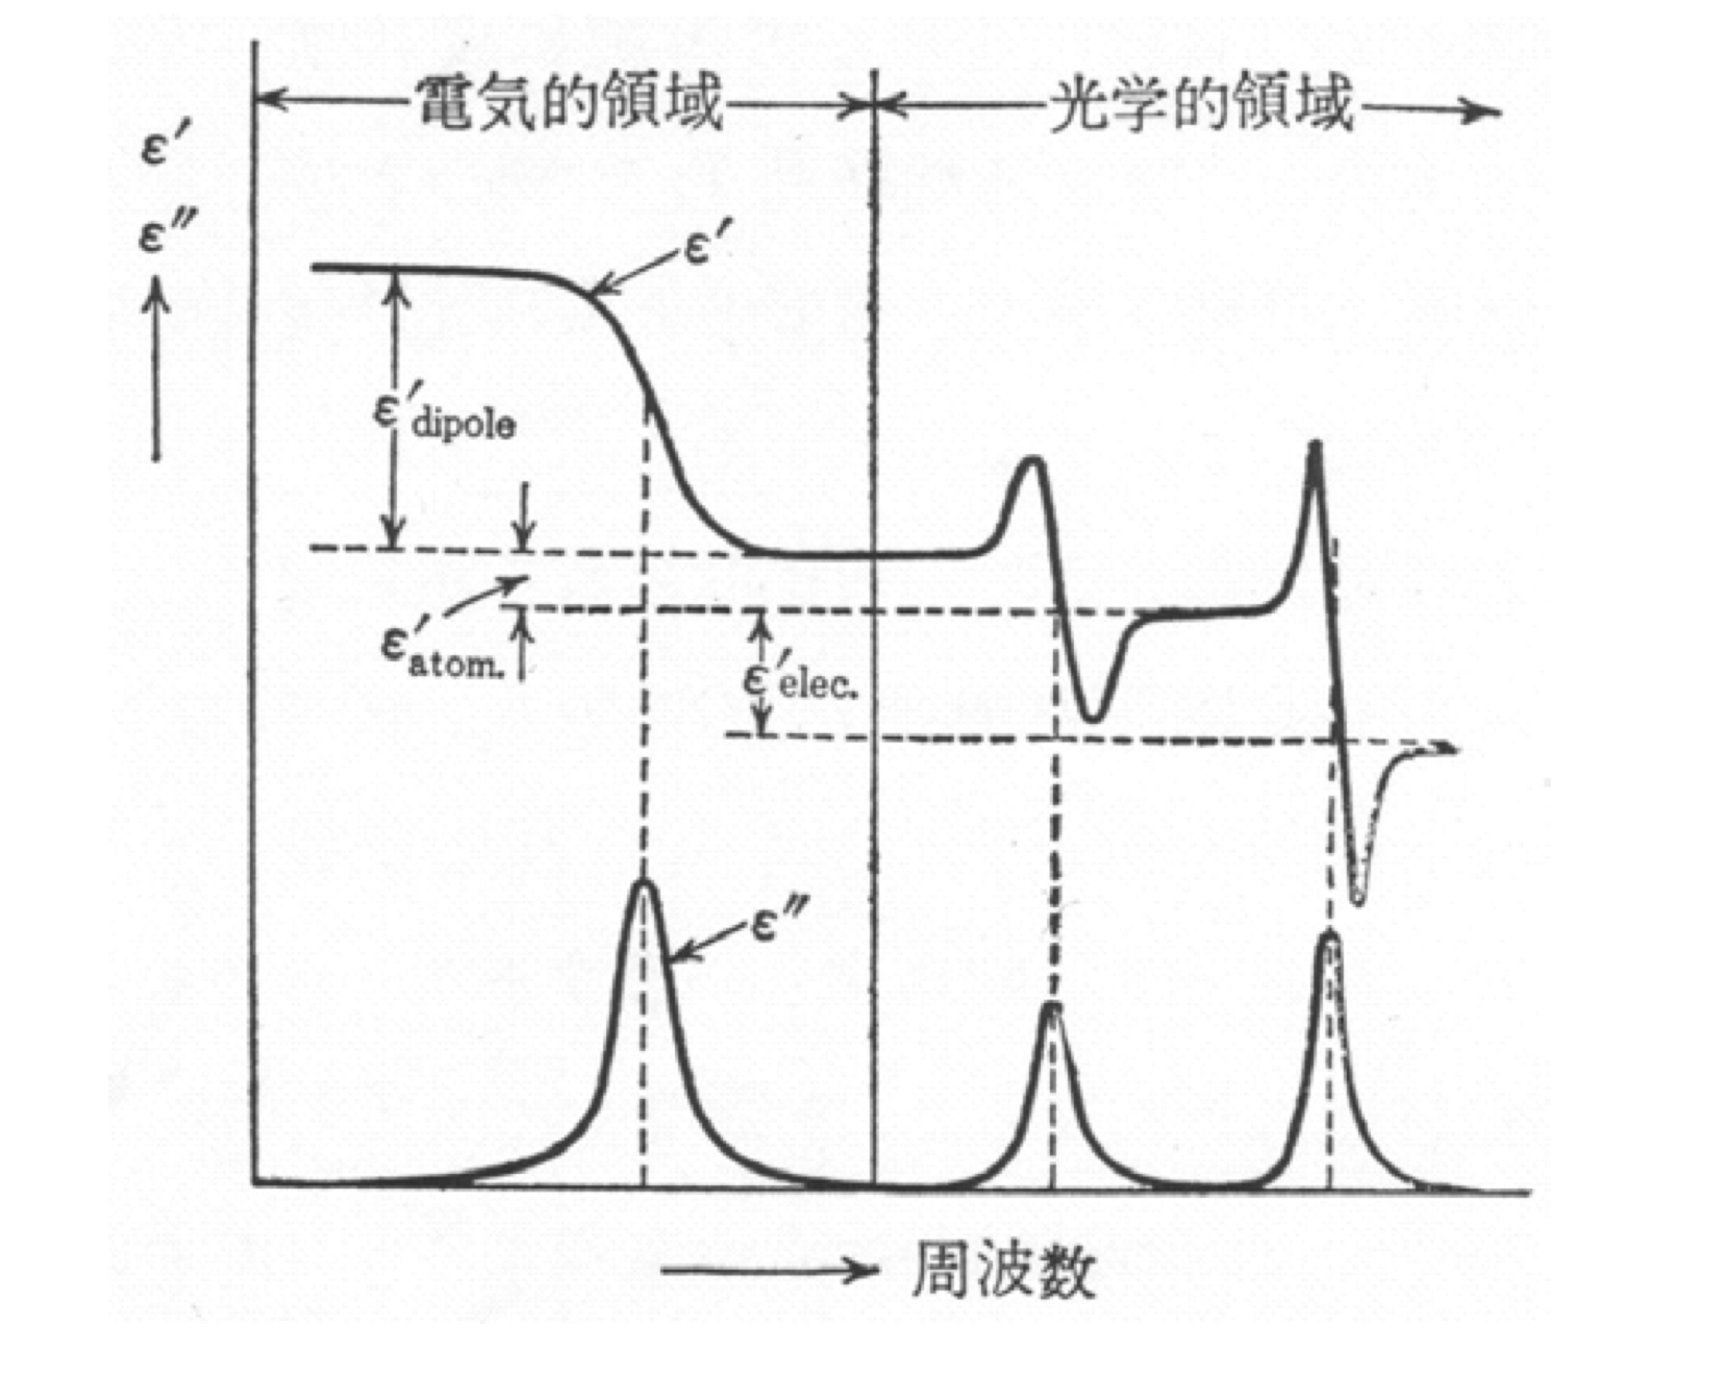
\includegraphics[width=1\linewidth]{fig/Diagram.pdf}
\caption{誘電率および誘電損率の周波数変化\\図中上、右から順に電子分極、イオン分極、配向分極の順で表している。誘電損率のピークは右から電子分極による赤外吸収、イオン分極による赤外吸収、配向分極による誘電緩和を表している。}
\label{fig:diagram}
\end{figurehere}
\subsection{\textrm{LCRメータ}}
実験で使用したLCRメータは、キャパシタンス実部$C'$と誘電体の損失角$\tan\delta$が計測できるように設計されている。
一方、本来計測したい値は、複素誘電率の実部$ε'$と虚部$ε''$である。これらの値は、式(1)を用いて、キャパシタンス実部$C'$と誘電体の損失角$\tan\delta$から計算することができる。
\begin{equation}
  ε_r^*=ε'-jε''=C'\frac{d}{ε_0S}-jC'\frac{d}{ε_0S}\tan\delta
\end{equation}
この式は、複素キャパシタンスの関係式$j\omega C^*=G+jB$と$C^*=ε_0ε_rS/d$から得られる。

\section{\textrm{Experimental procedures}}
\subsection{\textrm{LCRメータによる素子特性の測定}}
[使用器具] No.3の素子

周波数1Hzを開始とし、100kHzまでの交流電圧を印加し、抵抗、キャパシタ、インダクタの素子特性をLCRメータで測定した。\\
さらにブレッドボード上にRC直列回路を構成し、インピーダンスの実部と虚部の周波数依存性を観測した。\\

測定開始の前に、オープン回路、ショート回路を用いて、LCRメータの校正を行った。\\
\subsection{\textrm{PVAcフィルムの誘電率の周波数特性}}
PVAcフィルムをヒーターに貼り付け、周波数100を開始とし、100kHzの交流電圧を印加し、温度55℃、60℃、65℃、70の順に保温して、LCRメータで誘電率の周波数特性を測定した。\\
測定値として、インピーダンス実部Cと損失角$\tan\delta$を得た。\\

同様、測定開始の前に、オープン回路、ショート回路を用いて、LCRメータの校正を行った。\\

\section{\textrm{Results}}
\subsection{\textrm{単独素子の周波数特性}}
まず、抵抗の周波数特性をFig.2に示す。理論値は、$\theta=0$、$|Z|=const$となるはずであるが、高周波数になるにつれて、$\theta=0$と$|Z|$の規格値100 Ωからずれていることがわかる。\\
次に、インダクタの周波数特性をFig.3に示す。理論値は、$\theta=\frac{\pi}{2}$、$|Z|=j\omega L$となるはずであるが、低周波では$\theta\simeq 0$となっている。近似直線の傾きから、インダクタンスを求めると0.4625 mHとなった。規格値0.470 mHとの誤差は1.62\%であった。\\
キャパシタの周波数特性がFig.4である。理論値は、$\theta=-\frac{\pi}{2}$、$|Z|=\frac{1}{j\omega C}$となるはずである。位相のズレは然程大きくない。近似直線の傾きから、キャパシタンスを求めると9.506 μFとなった。規格値10 μFとの誤差は5.18\%であった。\\
最後に$RC$直列回路の周波数特性をFig.5に示す。$Z^* = R - j\frac{1}{\omega C}$の式の通り、周波数が大きくなるにつれ、インピーダンスの絶対値は抵抗R=100 Ωに漸近し、位相は0に近づいている。\\
\end{multicols}
\begin{figurehere}
\centering
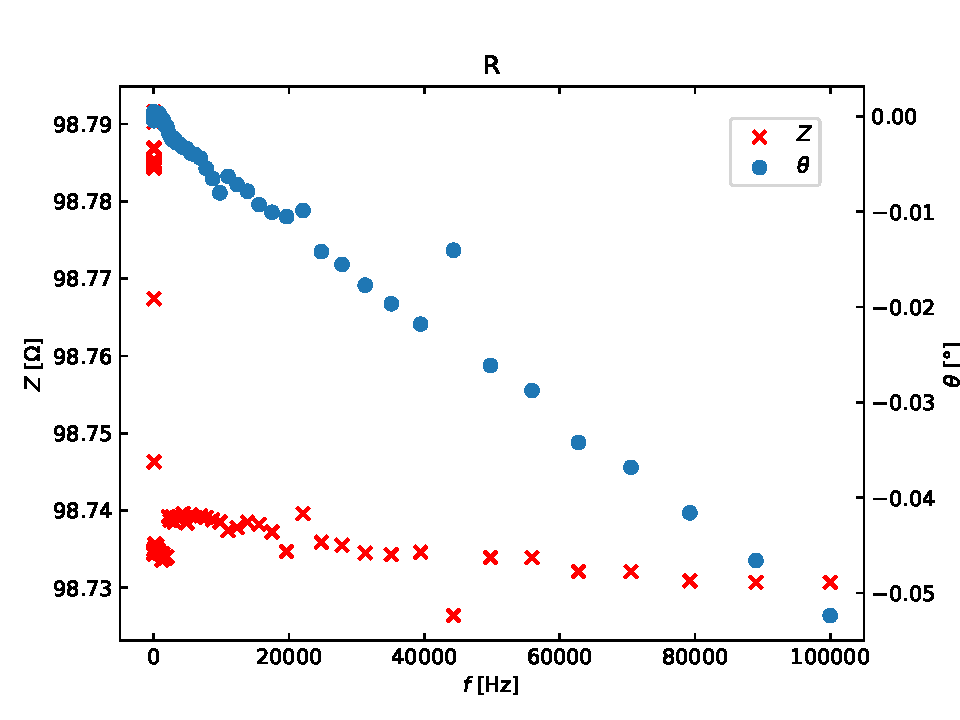
\includegraphics[width=0.5\linewidth]{fig/R.pdf}
\caption{Rの周波数特性}
\label{fig:C}
\end{figurehere}
\begin{figurehere}
\centering
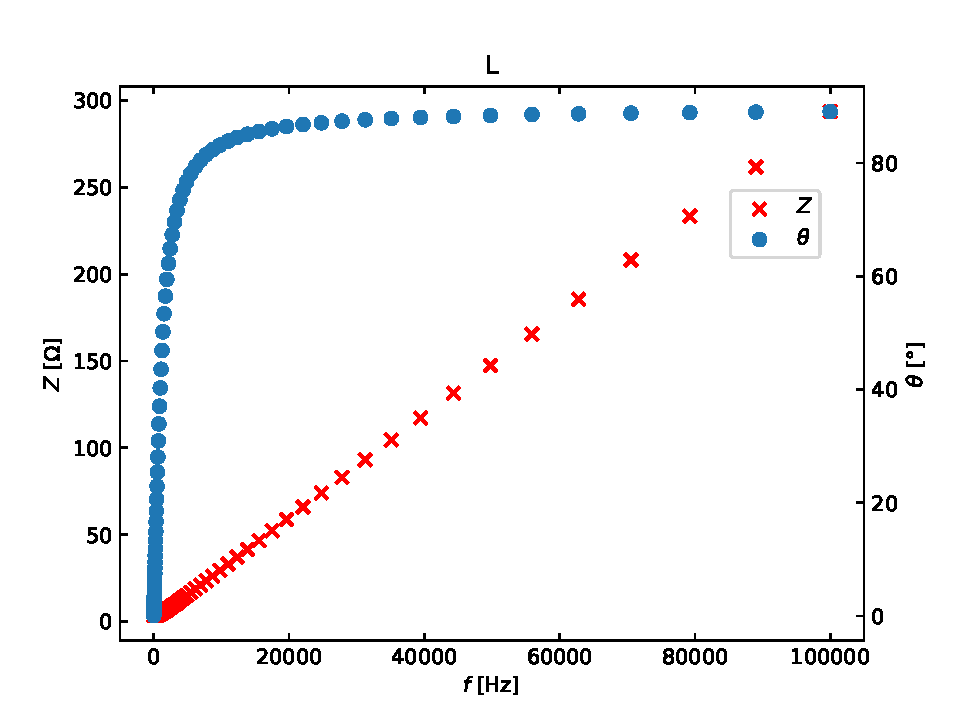
\includegraphics[width=0.5\linewidth]{fig/L.pdf}
\caption{Lの周波数特性}
\label{fig:L}
\end{figurehere}
\begin{figurehere}
\centering
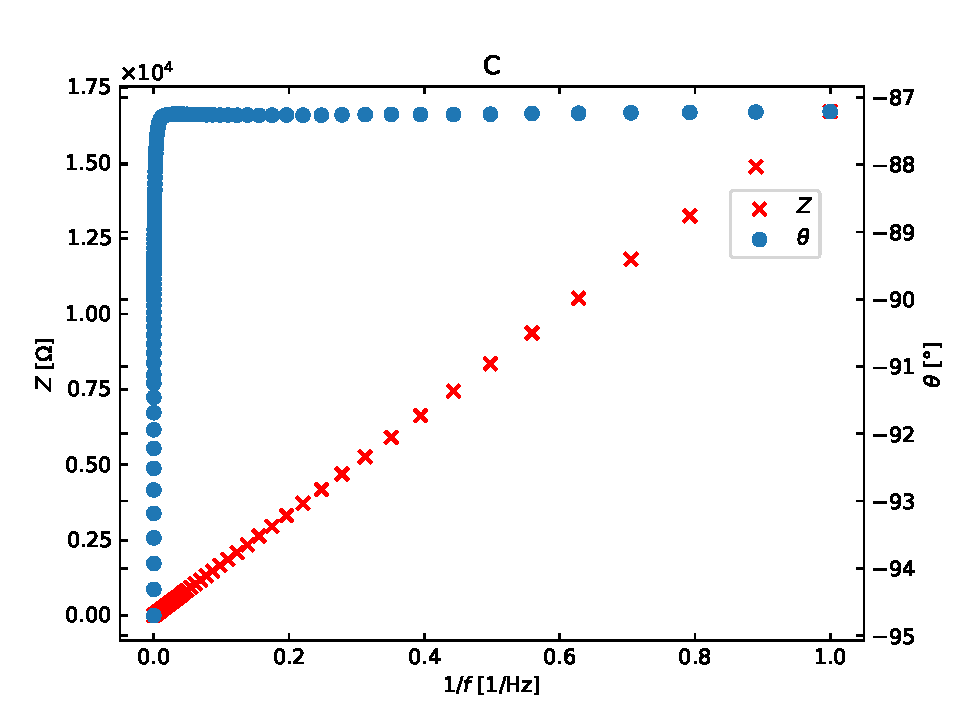
\includegraphics[width=0.5\linewidth]{fig/C.pdf}
\caption{Cの周波数特性}
\label{fig:C}
\end{figurehere}
\begin{figurehere}
\centering
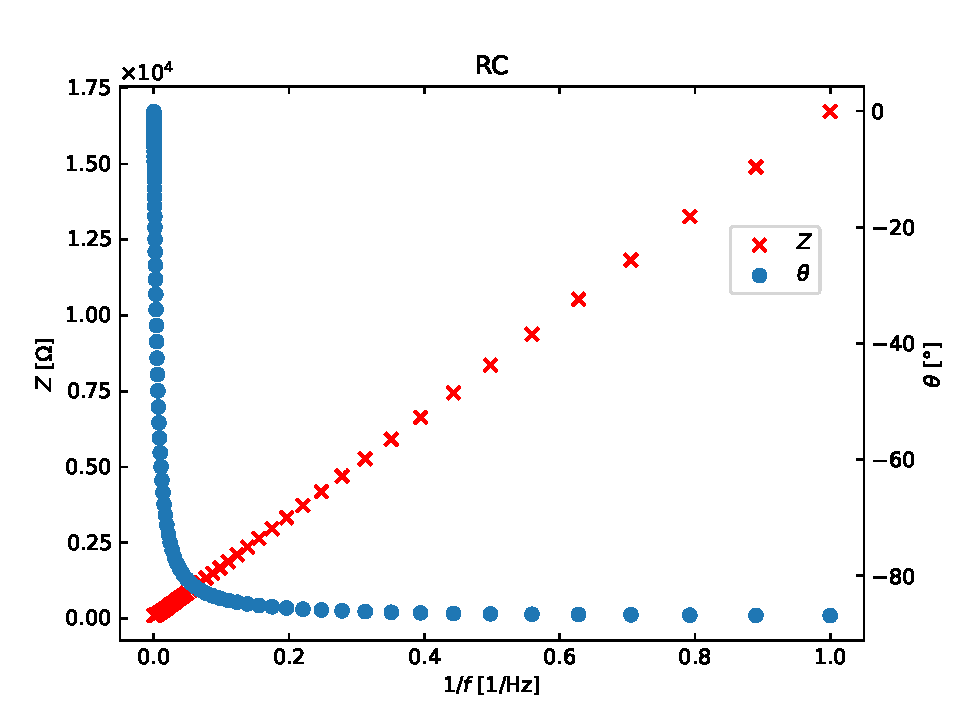
\includegraphics[width=0.5\linewidth]{fig/RC.pdf}
\caption{RC直列回路の周波数特性}
\label{fig:C}
\end{figurehere}
\subsection{\textrm{PVAcフィルムの誘電率の周波数特性}}
\begin{figurehere}
\centering
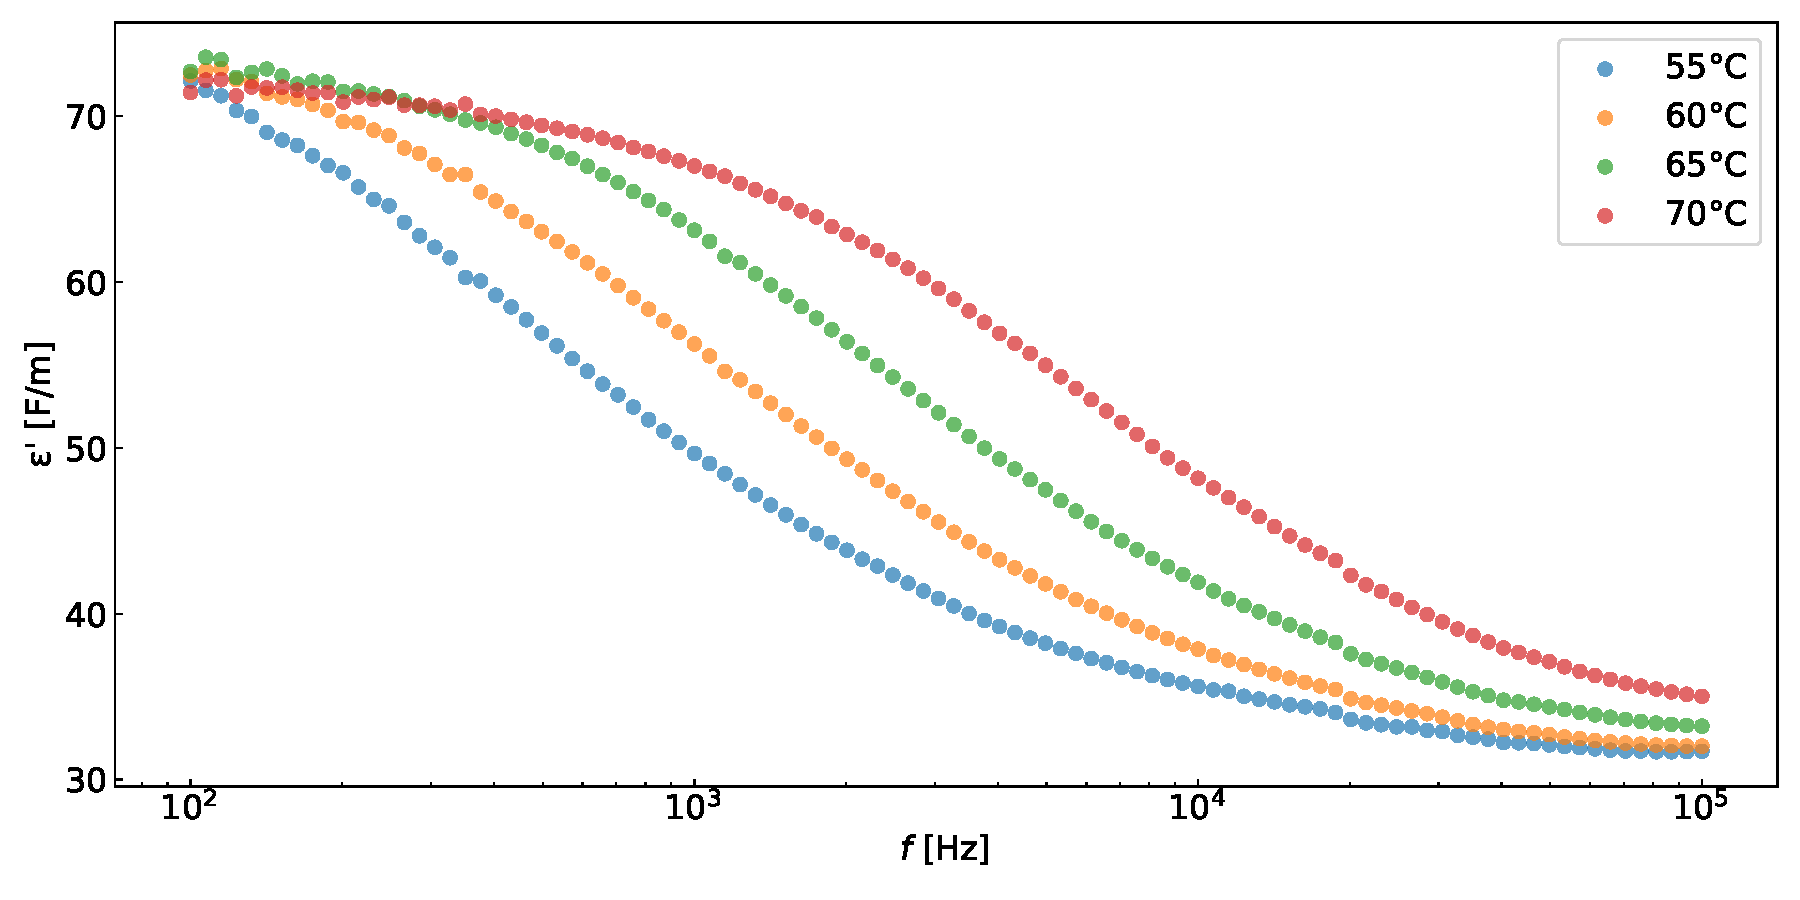
\includegraphics[width=0.7\linewidth]{fig/epsilon_prime.pdf}
\caption{PVAcフィルムの実部誘電率の周波数依存性}
\label{fig:epsilon_prime}
\end{figurehere}
\begin{figurehere}
  \centering
  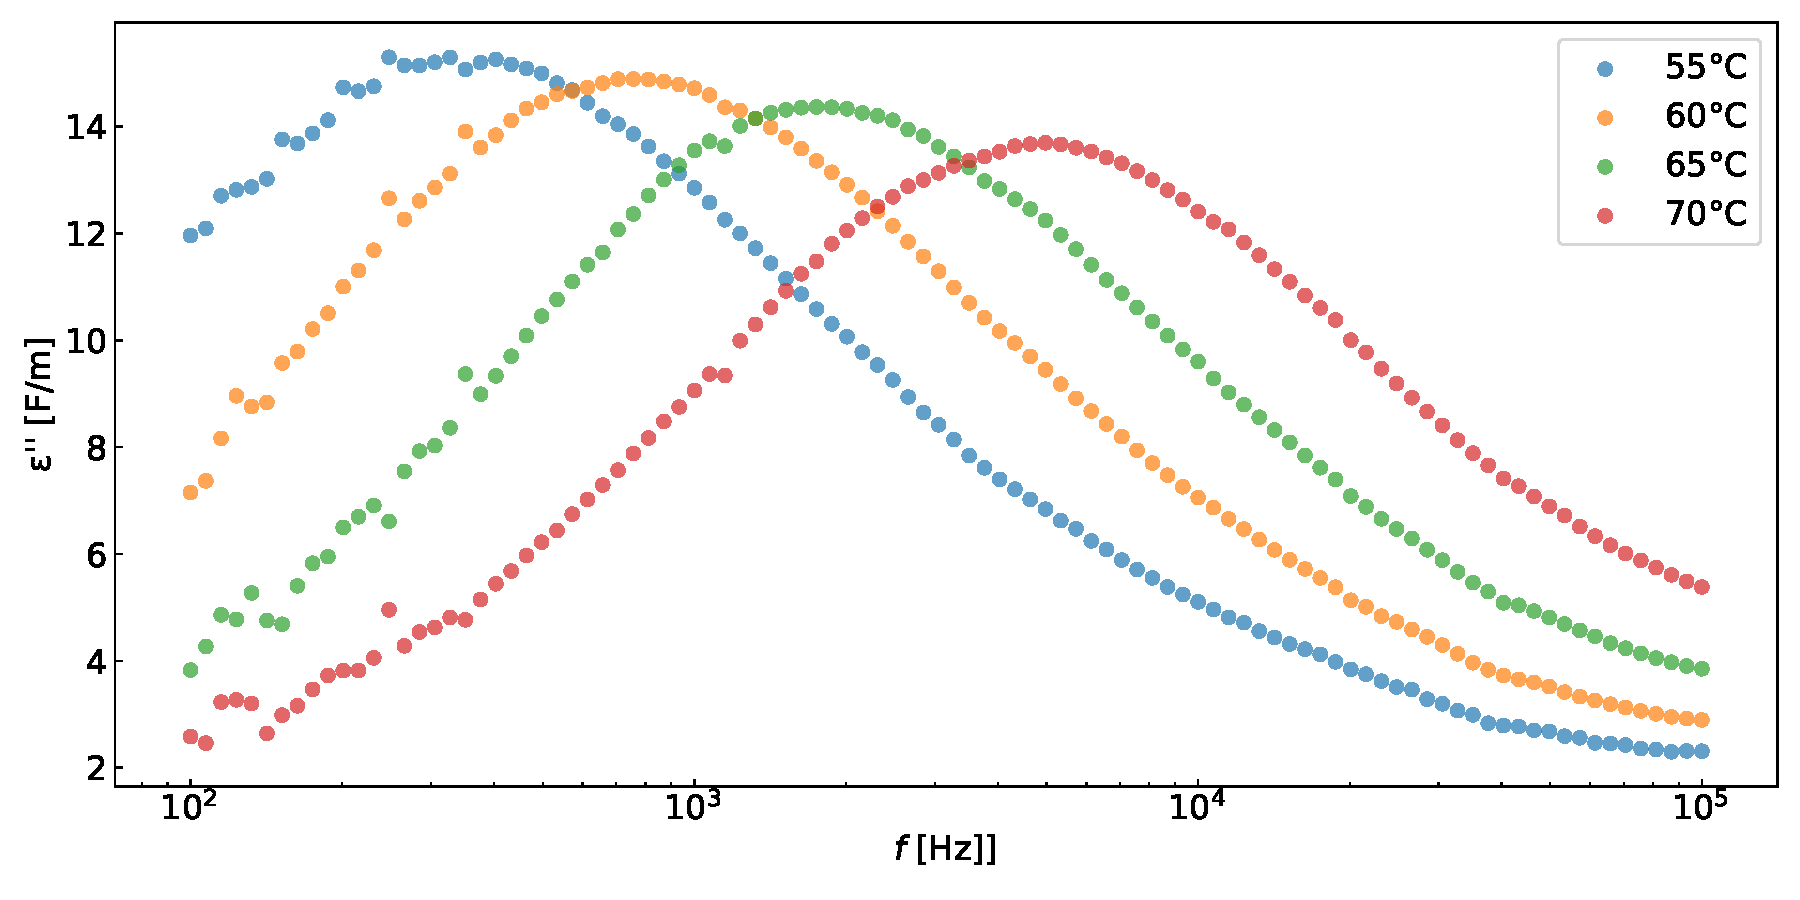
\includegraphics[width=0.7\linewidth]{fig/epsilon_double_prime.pdf}
  \caption{PVAcフィルムの虚部誘電率の周波数依存性\\青が55℃、黄が60℃、緑が65℃、赤が70℃の測定点を示している。}
  \label{fig:epsilon_prime}
  \end{figurehere}
\begin{multicols}{2}
LCRメータにより得られたインピーダンス実部$C'$と損失角$\tan\delta$を用いて、式(1)から、PVAcフィルムの誘電率の実部$ε'$と虚部$ε''$を計算した。\\
計算に用いた$d$、$S$、$ε_0$の値はTable.1に示す。
\begin{table}[H]
  \centering
  \caption{PVAcフィルムの誘電率の計算に用いたパラメータ}
  \begin{tabular}{lll}
    $d$ [m] & $S$ [$\text{m}^2$] & $\varepsilon_0$ [F/m] \\
    \midrule
    \midrule
    $200 \times 10^{-6}$ & $40 \times 10^{-6}$ & $8.85 \times 10^{-12}$ \\
  \end{tabular}
  \label{tab:addlabel}
\end{table}

Fig.6に、PVAcフィルムの実部誘電率の周波数依存性を示す。$f_r$は対数目盛で表示している。高周波数側になるにつれて$ε'$は減少していることが確認できる。これは、高周波数では、誘電体の配向分極が追従できなくなるため、誘電率が減少することによる。\\
また、温度が上昇するにつれて、$ε'$は増加していることがわかる。これは、温度が上昇すると、分子の運動エネルギーが増加し、配向分極が追従できなくなる周波数が増加するためである。\\
続いて、Fig.7にPVAcフィルムの虚部誘電率の周波数依存性を示す。$f_r$は対数目盛で表示している。いずれの温度においても、一つのピークを持つことがわかる。このピークは、配向分極が追従できなくなる緩和周波数を表している。また、温度が上昇するにつれて、緩和周波数が増加していることがわかる。これらの測定点を用いて、デバイの式(2)により緩和周波数を求めた。
\begin{equation}
  \epsilon(\omega) = \epsilon_\infty + \frac{{\epsilon_0 - \epsilon_\infty}}{{1 + j\omega\tau}}
\end{equation}
$\epsilon(\omega)$は角振動数$\omega$における誘電率、$\epsilon_\infty$は高周波極限における誘電率、$\epsilon_0$は低周波極限における誘電率、$\tau$は緩和時間$\frac{1}{2\pi f_r}$を表す。\\
$\epsilon_0$、$\epsilon_\infty$、$\tau$を最適化するようにフィッティングを行った結果をFig.9から12に示す。長くなったのでAppendixにまとめた。\\
赤線が、フィッティングにより得られたデバイの式の曲線であり、図中に最適化されたパラメータの値を示している。\\

\section{\textrm{Discussion}}
\subsection{\textrm{緩和周波数の温度依存性}}
デバイの式より求められた緩和周波数を横軸温度の逆数として、縦軸対数表示したものをFig.8に示す。
\begin{figurehere}
\centering
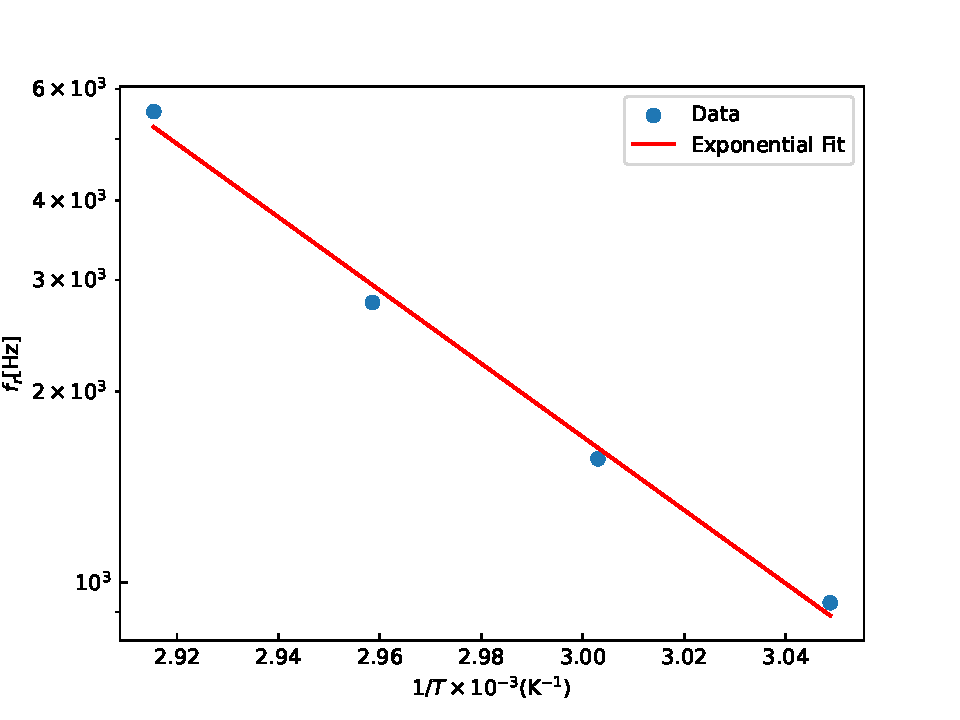
\includegraphics[width=1\linewidth]{fig/areniusu.pdf}
\caption{横軸を$\frac{1}{T}$、縦軸を$\ln{f_r}$として、線形フィッティングを行った結果}
\label{fig:fit_55}
\end{figurehere}

  
Fig.8をみると、緩和周波数は温度に依存しており、縦軸対数表示した際に、直線的に並んでいることが確認できる。これは、アレニウスの式で説明できる。
緩和周波数は、物質が外部の刺激(例えば、電場や力)にどれだけ迅速に反応するかを示す指標である。この反応速度は、アレニウスの式に従って温度に依存する。具体的には、温度が上昇すると、活性化エネルギーを越えることができる分子やイオンの割合が増加し、緩和周波数も増加する。
\begin{equation}
  f_r = A\exp{\frac{\Delta E}{RT}}
\end{equation}
$\Delta E$、$R$、$T$はそれぞれ、活性化エネルギー、気体定数、絶対温度を表す。
式()の両辺の対数をとると:
\begin{equation}
  \ln{f_r} = -\frac{1}{T}\frac{\Delta E}{R}\log_{10}{e} + a
\end{equation}
となる。
この式から、Fig.8の近侍直線の傾きは、$-\frac{\Delta E}{R}\log_{10}{e}$に相当する。この傾きを求めることで、活性化エネルギーを求めることができる。
$R=8.314$J/(mol・K)を代入して計算すると、$\Delta E$の計算結果は:
\begin{equation}
  \Delta E \simeq 3.65 \times 10^5  \text{J/mol}
\end{equation}
となった。
\subsection{\textrm{RC直列回路のインピーダンスの実部、虚部の周波数依存性}}
\begin{figurehere}
\centering
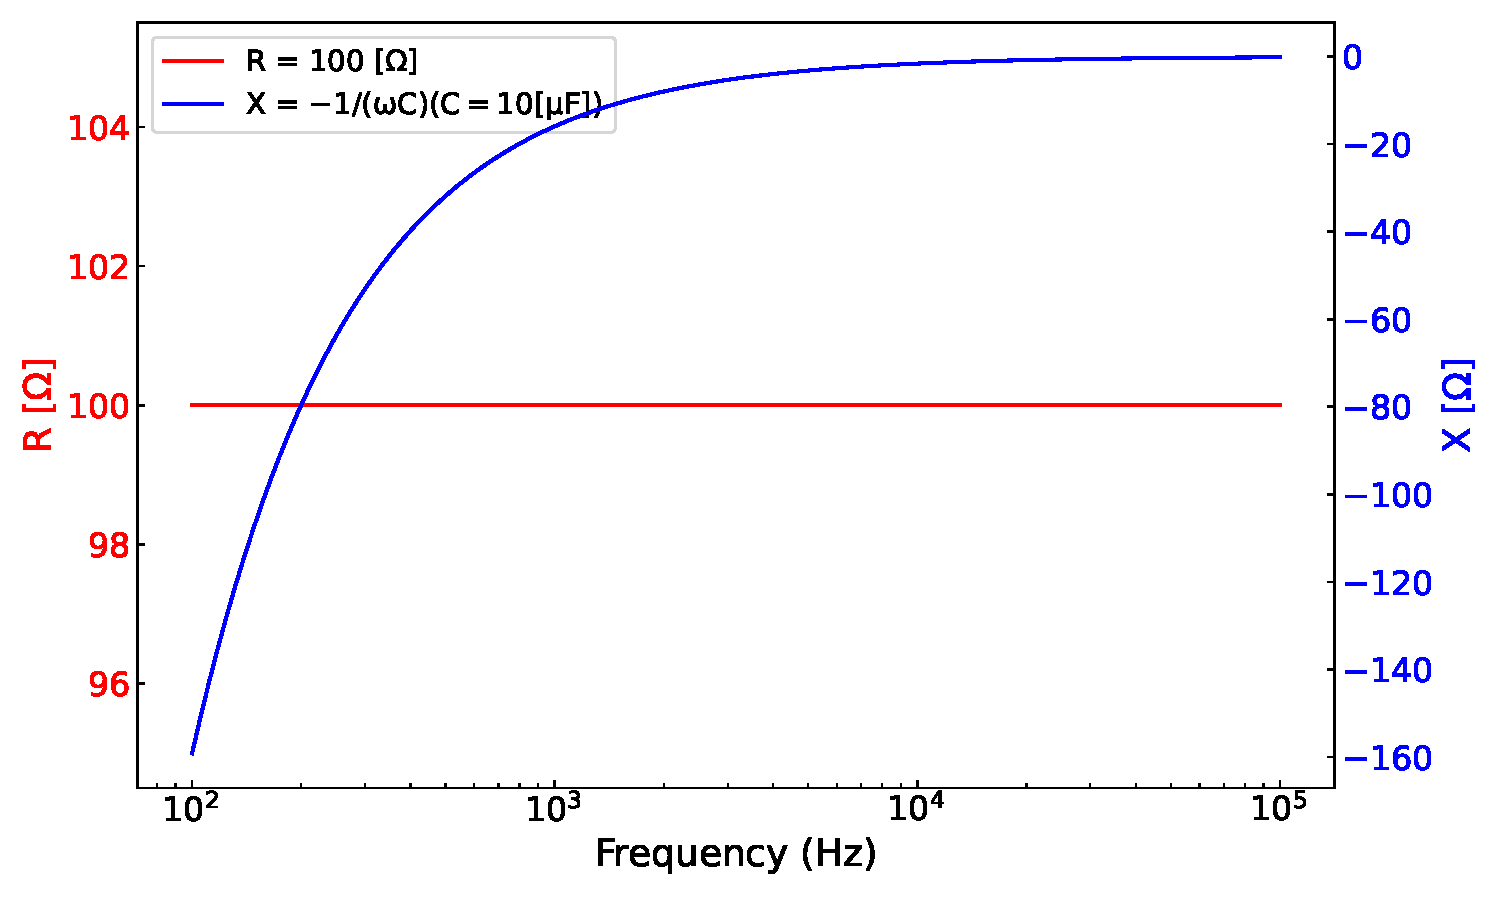
\includegraphics[width=1.1\linewidth]{fig/rc_impedance.pdf}
\caption{RC直列回路の等価回路}
\label{fig:rc_theorical}
\end{figurehere}
\subsection{\textrm{RC直列回路のアドミッタンスの実部虚部の周波数依存性}}
合成アドミッタンス:
\begin{align} 
  Y^* = G + jB&&
     = \frac{(\omega C)^2R}{1 + (\omega CR)^2} + j\frac{\omega C}{1 + (\omega CR)^2}
\end{align}
に$C = 10μF$、$R = 100Ω$を代入した、合成アドミッタンスの実部と虚部の周波数依存性をFig.10に示す。

\begin{figure}[H]
  \centering
  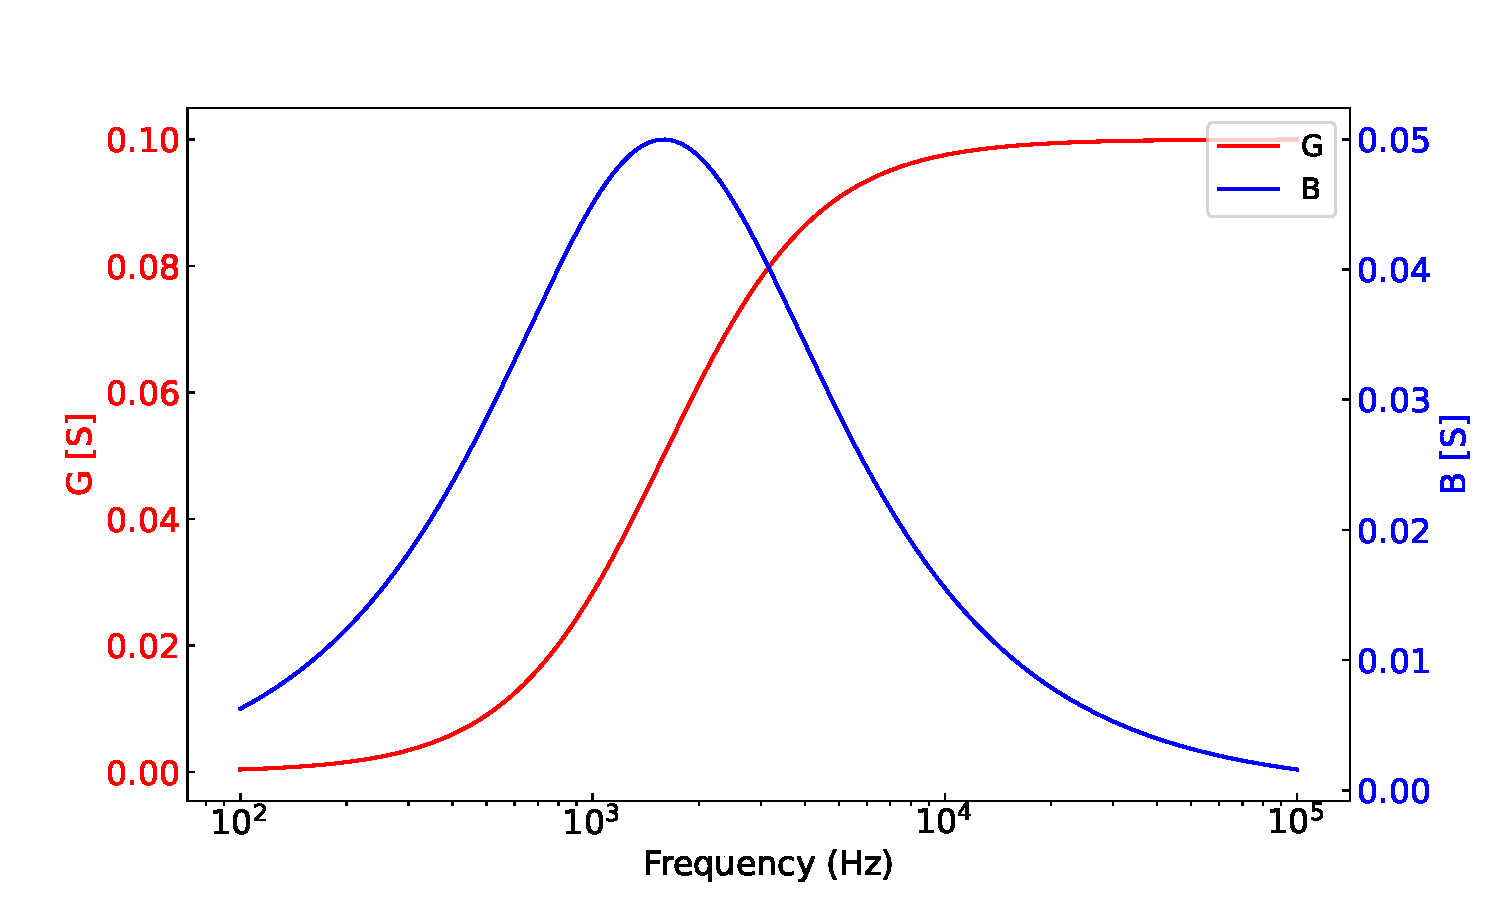
\includegraphics[width=1.1\linewidth]{fig/rc_admittance.pdf}
  \caption{RC直列回路のインピーダンスの実部と虚部の周波数依存性}
  \label{fig:combined_graph}
\end{figure}
$Y^*=j\omega C^*$の関係から、(6)式の両辺を$j\omega$で割ると:
\begin{equation}
  C^* = \frac{C}{1 + (\omega CR)^2} - j\frac{\omega C^2R}{1 + (\omega CR)^2}
\end{equation}
となり、RC直列回路を一つのキャパシタに見立てた時の$C^*$が得られる。\\
(7)式の$C^*$の実部虚部の周波数依存性Fig.11に示す。
Fig.11は、PVAcフィルムの誘電率の周波数特性と一致していることがわかる。すなわち、RC直列回路はPVAcフィルムの誘電緩和を表す等価回路であると言える。

\begin{figure}[H]
  \centering
  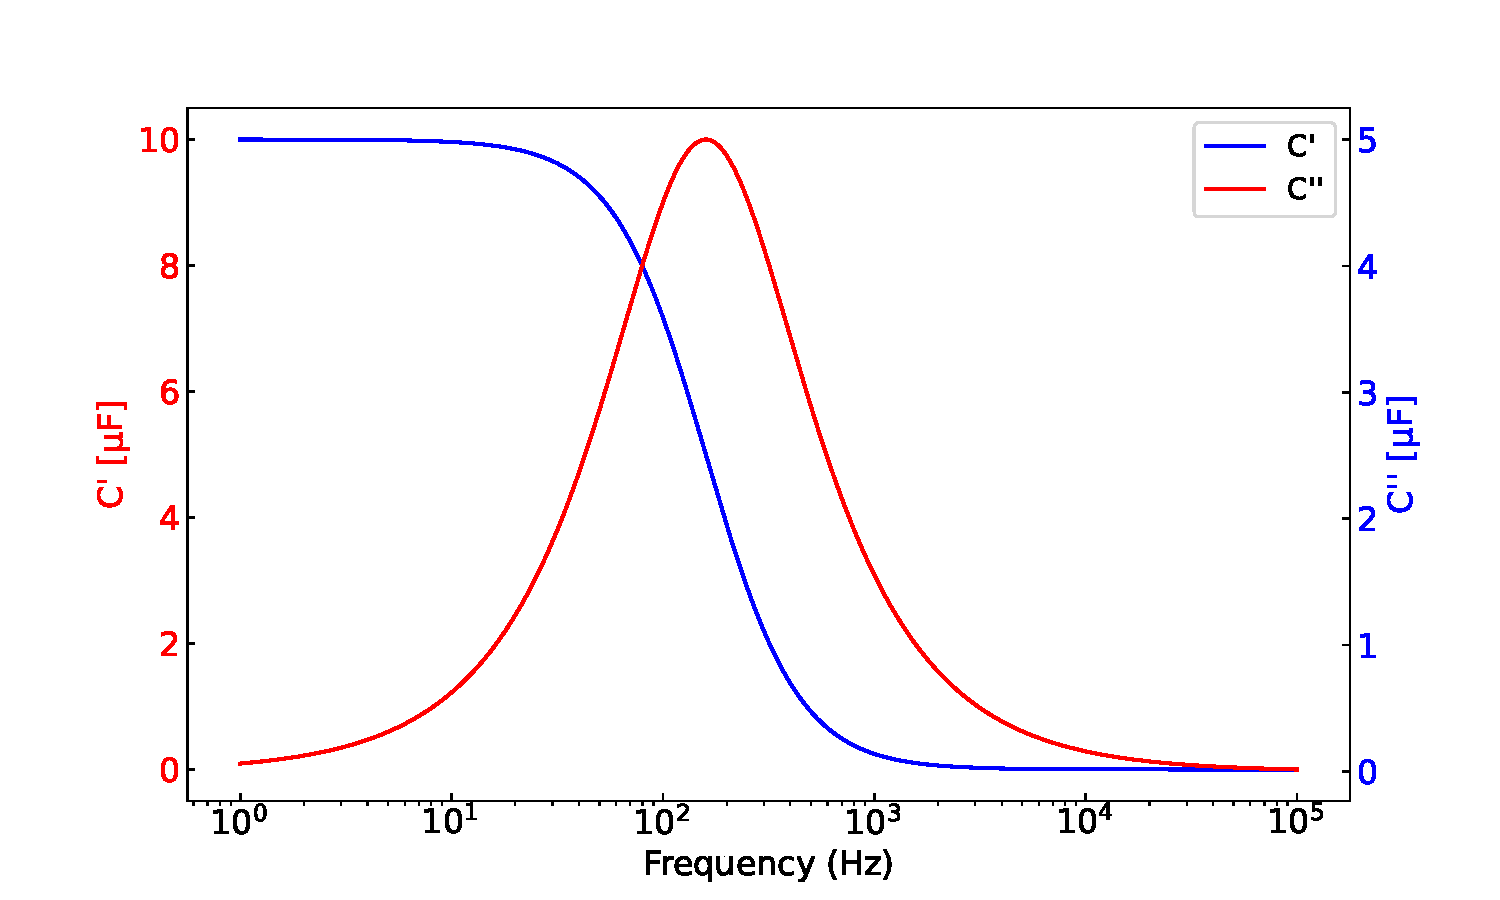
\includegraphics[width=1.1\linewidth]{fig/rc_capacita.pdf}
  \caption{RC直列回路のインピーダンスの実部と虚部の周波数依存性}
  \label{fig:combined_graph}
\end{figure}

\subsection{\textrm{LCRメータの導線間に生じる並列コンデンサーの影響}}
理論上、純粋な抵抗素子では位相角$\theta$は周波数に依存せず0°で一定である。しかしながら、Fig.2の測定結果を見ると、高周波数になるにつれて、位相角θが減少することが確認された。これは、LCRメータの導線間に並列に存在するコンデンサーの影響を受けているためである。\\
LCRメータの測定回路において、抵抗$R$だけでなく、導線間に寄生容量が現れる。\\
寄生容量$C$を含む抵抗$R$の並列回路の合成インピーダンス$Z$は次式で表される:
\begin{equation}
  Z = \frac{1}{\frac{1}{R}+j2\pi fC}
\end{equation}
インいーダンス$Z$の実部虚部から、位相角$\theta$を求めると:
\begin{equation}
 {\theta} = \tan^{-1} (-2\pi fRC)
\end{equation}
となる。\\
$\theta$が小さな角度の時は、$\tan{\theta} \simeq \theta$と近似できるため、位相角$\theta$は:
\begin{equation}
  \theta \simeq -2\pi fRC
\end{equation}
となり、$f$に比例して減少することがわかる。\\
Fig.2の近似直線の傾きを求めることで、寄生容量$C$を求めることができる。\\
Fig.2の近似直線の傾きを求めると、$-5.197\times 10^{-7}$となった。従って:
\begin{equation}
  -5.197\times 10^{-7} = -2\pi \times 100 \times C
\end{equation}
ここから、寄生容量$C$を解くと:
\begin{equation}
  C = 8.27 \times 10^{-13} \text{F}
\end{equation}
従って、$C = 0.827$ pFとなった。\\

\section{\textrm{Conclusion}}
この実験で得られた結論は以下の通りである:\\
抵抗の位相角は高周波数になるにつれて減少することが確認された。これは、LCRメータの導線間に並列に生じるコンデンサーの影響が原因であると考えられる。\\
抵抗の$\theta$-$f$のグラフの測定点から近似直線をひき、その傾きから寄生容量を求めると、$C=0.827$ pFとなった。\\
さらに、PVAcフィルムの誘電率の周波数依存性を測定し、誘電緩和現象を観測した。温度が上昇するにつれて、緩和周波数が増加することを確認した。\\
また、RC直列回路のインピーダンスの実部と虚部の周波数依存性のグラフとPVAcフィルムの誘電率の周波数依存性のグラフを比較すると、これらの特性が同じ特性曲線を示すことを確認した。
この結果から、RC直列回路がPVAcフィルムの誘電緩和を表す等価回路であることが示唆された。
\begin{thebibliography}{文献数}
  \bibitem{ID} 東京理科大学理学部応用物理学科, ``物理学実験テキスト'', 2023.
  \end{thebibliography}
\clearpage
\section{\textrm{Appendix}}
\end{multicols}
\begin{figurehere}
  \centering
  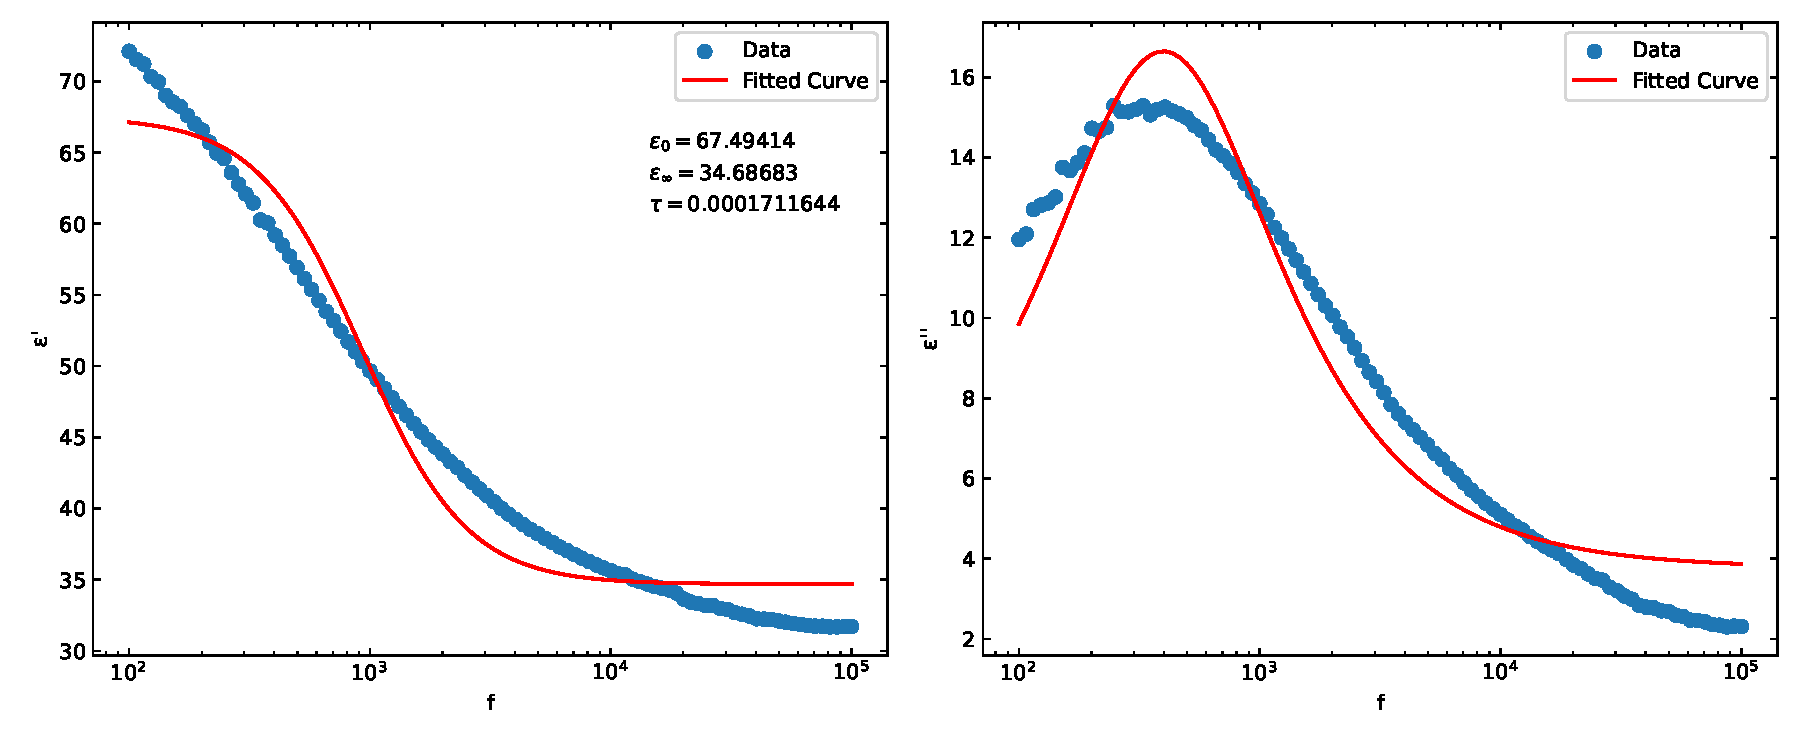
\includegraphics[width=0.9\linewidth]{fig/fit_55.pdf}
  \caption{55℃におけるPVAcフィルムの誘電率の周波数依存性}
  \label{fig:fit_55}
  \end{figurehere}
  \begin{figurehere}
  \centering
  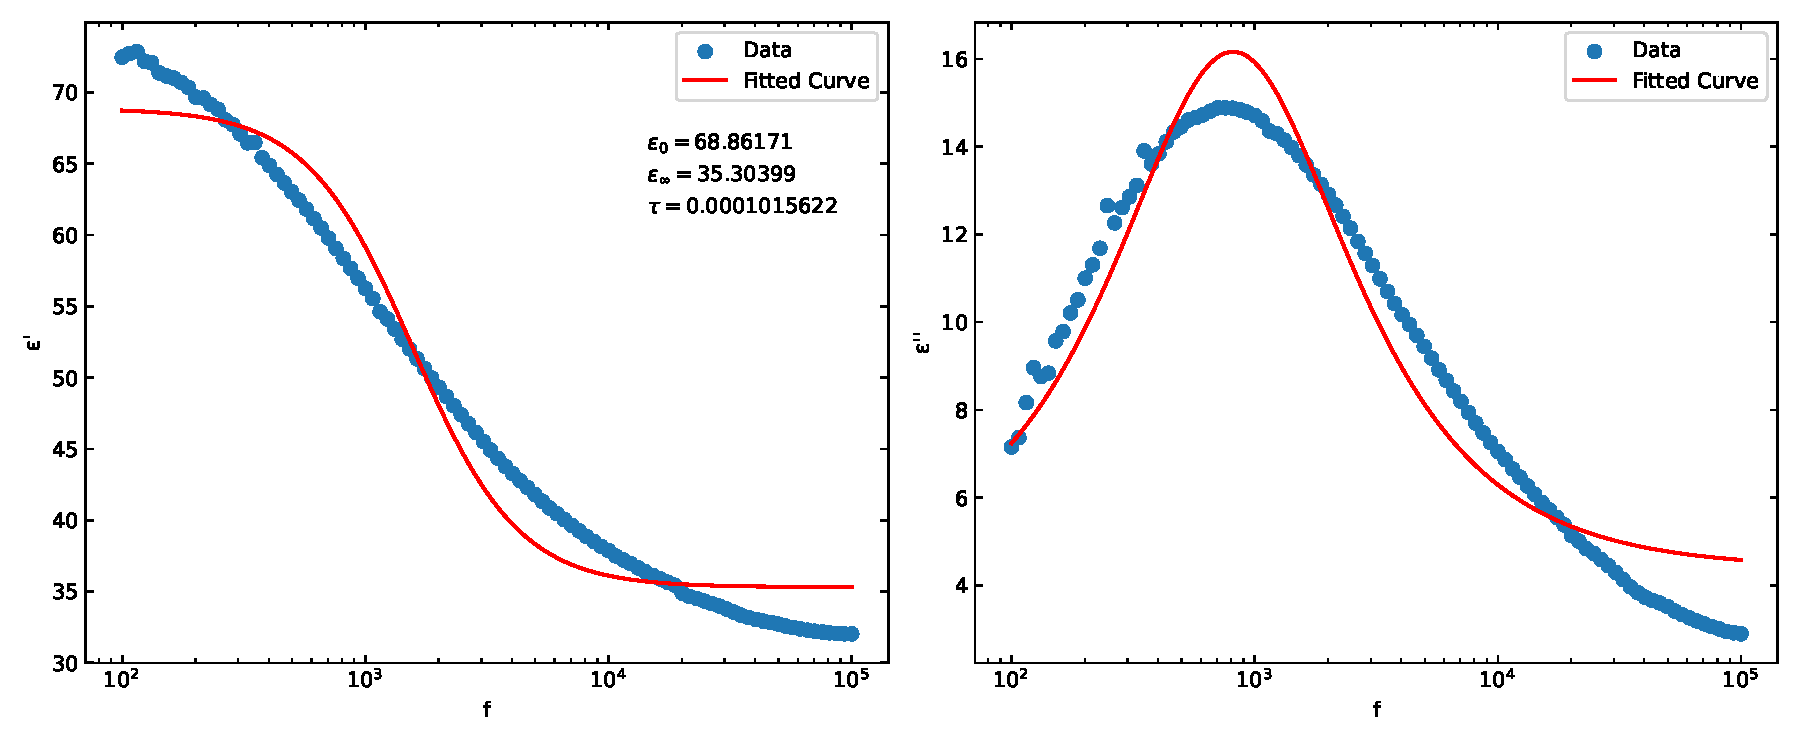
\includegraphics[width=0.9\linewidth]{fig/fit_60.pdf}
  \caption{60℃におけるPVAcフィルムの誘電率の周波数依存性}
  \label{fig:fit_55}
  \end{figurehere}
  \begin{figurehere}
  \centering
  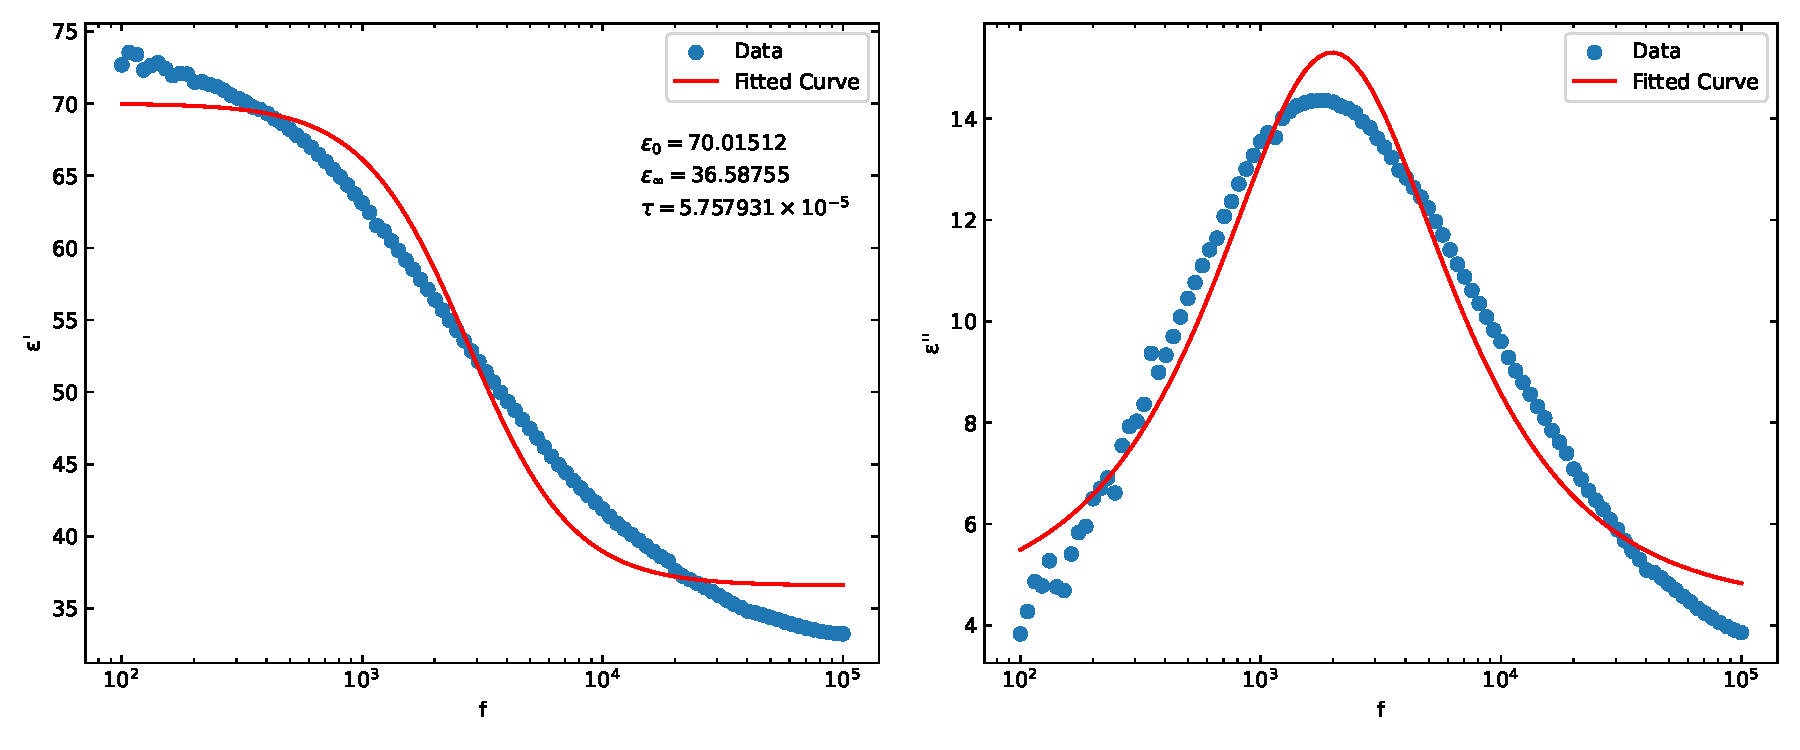
\includegraphics[width=0.9\linewidth]{fig/fit_65.pdf}
  \caption{65℃におけるPVAcフィルムの誘電率の周波数依存性}
  \label{fig:fit_55}
  \end{figurehere}
  \begin{figurehere}
  \centering
  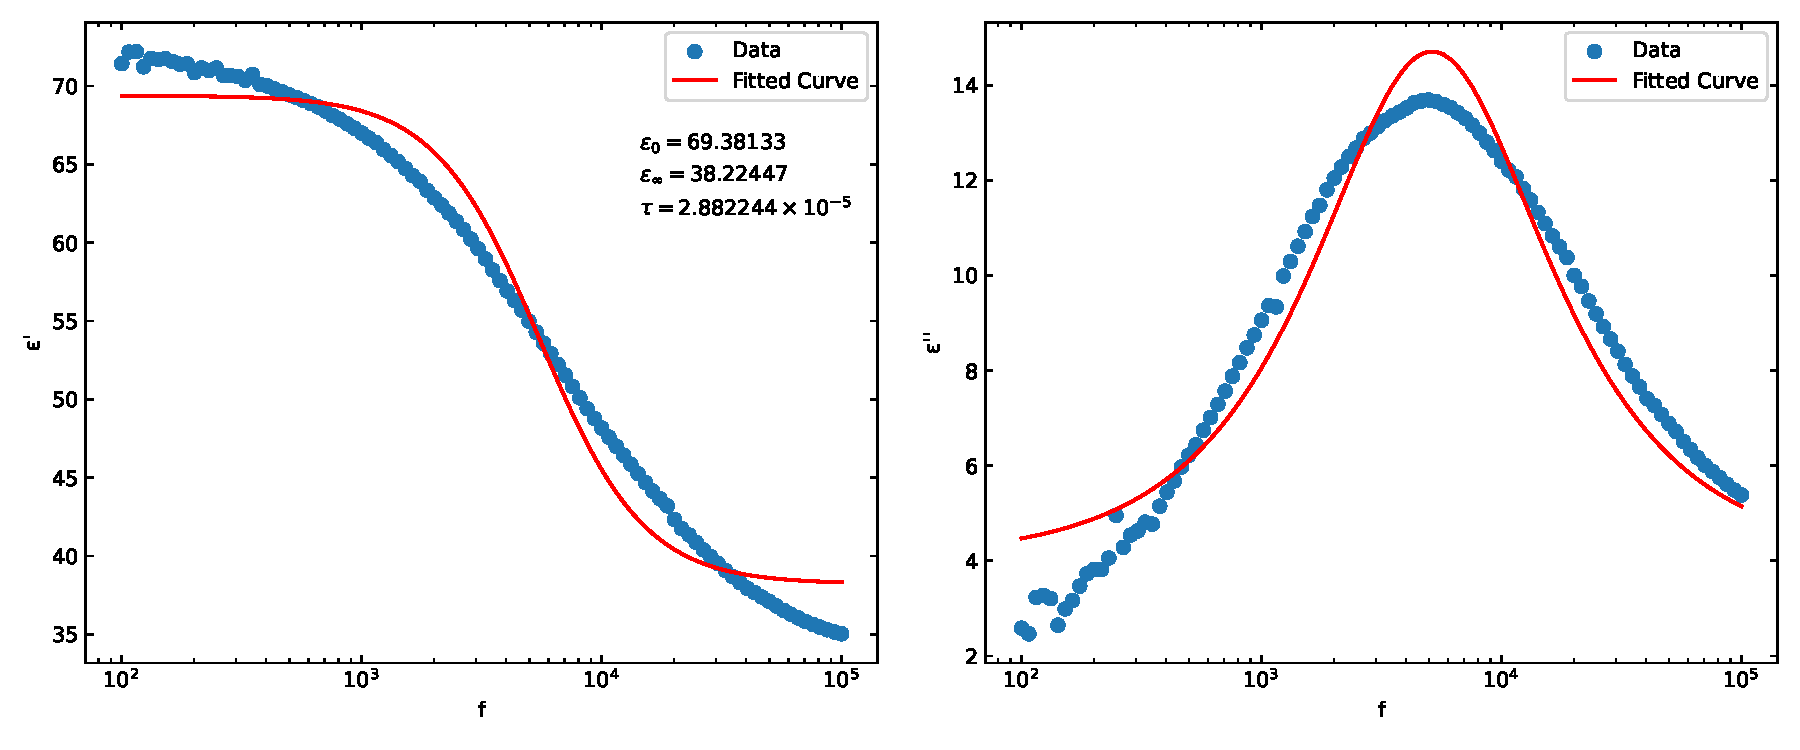
\includegraphics[width=0.9\linewidth]{fig/fit_70.pdf}
  \caption{70℃におけるPVAcフィルムの誘電率の周波数依存性}
  \label{fig:fit_55}
  \end{figurehere}



\end{document}